\section{Contextualization} \label{sec:context}

% Context (what is the importance of time series forecasting?)
Time series forecasting is an essential approach for businesses and researchers to make informed decisions by predicting future trends and patterns in a given time series data. Moreover, it plays a critical role in diverse fields, such as business planning and strategy, resource optimization, risk management, financial planning, marketing and sales, among others. Time series forecasting plays a significant role in business planning, as it helps predict future trends and patterns in sales and other key business metrics. This information is critical for businesses to make strategic decisions, such as when to launch new products or services, allocate resources, and manage their supply chain \cite{ma2021Retail}. Also, it could optimize companies' resources by predicting demand patterns and identifying potential bottlenecks. Those companies can use this information to allocate personnel, inventory, and equipment more efficiently and reduce costs.

Furthermore, by predicting future events, such as natural disasters or economic downturns, businesses could take advantage of the use of time series forecasting as they can take steps to mitigate the impact of these events and keep their operations running smoothly. This strategy also encompasses government and public policy regarding public health, sanitation, and well-being \cite{ribeiro2020Shortterm}. Additionally, time series forecasting is essential in financial planning. It can help forecast trends and changes in the stock market, interest rates, and other economic factors making it critical for businesses and investors to make reasoned decisions and stay ahead of the competition \cite{dasilva2020Multistep}. Last, time series forecasting is also handy for marketing and sales teams, as it helps predict demand and consumer behavior. In this way, they can make informed decisions on pricing, promotions, and customer targeting, which can help increase sales and revenue \cite{sohrabpour2021Export}.

% The methods explored (what are primary methods used in time series forecasting? ARIMA, statistical methods)
Generally, to forecast time series, statistical approaches have been massively used. In particular, Box \& Jenkins method \cite{box2016Time} applies \ac{ARMA} or \ac{ARIMA} models to find the best fit of a model to past values of a time series. Moreover, there is the Holt-Winters algorithm \cite{holt2004Forecasting, winters1960Forecasting}, exponential smoothing \cite{brown1961Fundamental}, Na\"ive approaches \cite{ribenboim1979Naive}, Croston's method \cite{croston1972Forecasting}, and epidemiological models, such as \ac{SIR} models \cite{kermack1927Contribution}, among others.

% Challenges (why is it difficult to forecast time series accurately?)
Nevertheless, forecasting time series accurately can be challenging. One reason is the complexity of the time series data, making it difficult to interpret. The data may be noisy, with many different patterns and trends that can make identifying the underlying patterns and relationships challenging. Also, real-world time series generally present high fluctuations and nonlinear and non-stationary behavior \cite{stepchenko2017Nonlinear, tealab2017Forecasting}. These characteristics mostly lead to imprecise predictions by the statistical models, which could not follow the data extremes and learn from the changes in the data pattern. These imprecise predictions result in low accuracy and, consequently, high forecasting errors.

% The use of AI (why is AI an efficient method for time series forecasting?)
To overcome this drawback, \ac{AI} models are proposed for time series forecasting once they can capture the complex and nonlinear relationships in time series data. These models can identify patterns and relationships that may not be immediately apparent by traditional statistical methods. Further, \ac{AI} models can learn and adapt to new data over time, improving their accuracy and effectiveness. Based on this ability to adapt and learn, it is possible to highlight the field of machine learning models. Machine learning is a subset of \ac{AI} that focuses on developing algorithms to learn and make predictions based on data. Also, machine learning involves training a model on a large data set and then using that model to make predictions or decisions about new data. Machine learning algorithms can be classified into supervised, unsupervised, and reinforcement learning. Figure~\ref{fig:ml_path} presents the roadmap from the study areas from \ac{AI} to time series forecasting.

\begin{figure}[htb!]
    \centering
    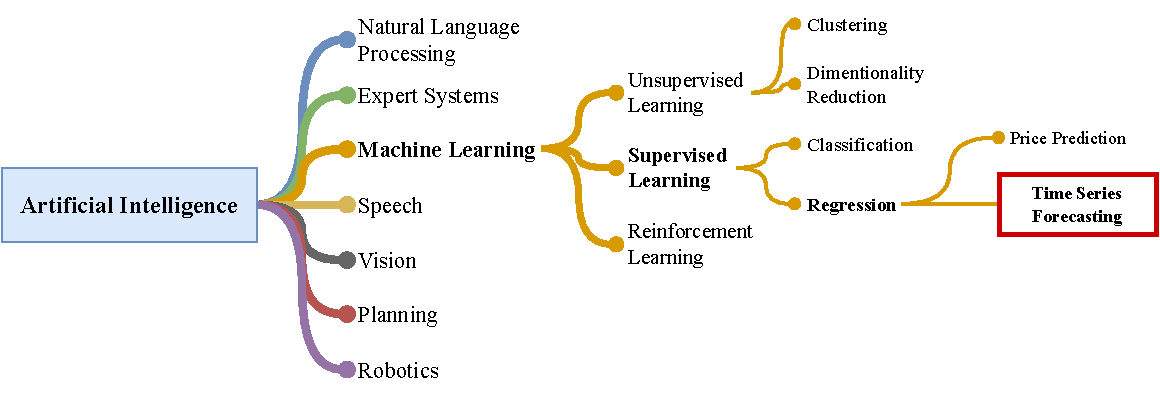
\includegraphics[width=\linewidth]{Media/roadmap.pdf}
    \caption{Time series forecasting roadmap}
    \label{fig:ml_path}
    \source{Author (2023)}
\end{figure}

% The Hybrid approaches (why hybrid methods could be more interesting than single AI models?)
\ac{AI} models have been effectively used in diverse fields of study, such as sustainable water resources management \cite{niu2021Evaluating}, health care and hospital administration \cite{piccialli2021Artificial}, load forecasting \cite{hou2022Review}, supply chain management \cite{mediavilla2022Review}. Besides, the hybridization of forecasting methods has been widely studied to enhance the accuracy of time series forecasting. This hybrid approach usually involves combinations such as signal decomposition methods \cite{song2022Application}, optimization algorithms \cite{jiang2023Multivariable}, and ensemble learning approaches \cite{ribeiro2023Cooperative}. In general, hybrid approaches perform better than single forecasting models, primarily due to the diverse characteristics of each employed approach which help each other in identifying the data pattern and behavior, even in nonlinear and high fluctuation data.

% The stacking-ensemble learning advantage (why using stacking-ensemble learning better than other approaches? Compare it to the different ensemble approaches, cite the divide-and-conquer strategy)
Regarding the ensemble learning models cited above, it is possible to divide them into three categories: bagging, boosting, and stacking \cite{das2022Comparison}.
%
The Bagging Ensemble Learning approach (also called bootstrap aggregation) aims to decrease the variance of the forecasting model by generating multiple versions of the original data, with replacement, and using them to obtain an aggregated predictor. The arithmetic average of the synthetic sample predictions obtains the prediction of the bagging approach. 
%
The Boosting Ensemble Learning approach combines a set of sequenced weak models to obtain a high-accuracy model. It aims to reduce the bias, improving the model's suitability to data. It learns from the errors of the previous model iteratively by increasing the importance of those errors in future iterations.
%
The \ac{STACK} approach stands out due to its learning structure composed of layers to increase the learning process by combining diverse methods in one layer and another more robust model in a consequent layer (details in Chapter \ref{chap:theoretical}). This feature allows users to develop a more robust forecasting model from the well-known \ac{AI} models. Also, this approach takes advantage of the divide-and-conquer principle by using the best characteristic of each model used in its layer to potentialize the learning process, consequently improving the accuracy of the proposed model.

% The signal decomposition strategy (how could signal decomposition preprocess the data and make the learning process more manageable?)
Moreover, the other practical approach to hybridization is the signal decomposition model. The signal decomposition approach aims to preprocess the data into subsets of the original data \cite{zhou2022Empirical}, removing the noise of the data and making the learning process easier. Each signal decomposition model has its strategy to derivate the data. For example, \ac{STL} extracts the seasonal and trend features from the data, or \ac{EWT} which divides the Fourier spectrum of the signal into continuous intervals, then construct wavelet filter banks on each interval for filtering, and finally obtain a group of components \cite{fan2023Shortterm}. This derivation allows the forecasting model to learn the pattern of the denoised subsets and then reconstruct the signal to obtain the final prediction \cite{moreno2018Wind}. Once the signal decomposition models can transform any time series, this strategy becomes handy when dealing with noisy, nonlinear, non-stationary ones.

% The hypothesis
Based on the previous discussion, this thesis hypothesizes: can the combination of multi-stage decomposition strategy with a stacking-ensemble learning approach improve the accuracy of forecasting models applied in real-world time series?